\section{Theorie}
\label{sec:Theorie}
\subsection{Zielsetzung}
In diesem Versuch wird mit Hilfe von Röntgenstrahlung
das Emissionsspektrum einer
Cu-Röntgenröhre bestimmt. Außerdem werden die Absorptionsspektren verschiedener
Materialien untersucht.

\subsection{Emission von Röntgenstrahlung}
Wenn Elektronen in einer evakuierten Röhre aus einer Glühkathode ausgelöst und
dann zur Anode beschleunigt werden, wo sie auf das Anodenmaterial treffen, entsteht
Röntgenstrahlung. Diese besteht aus dem kontinuierlichen Bremsspektrum und dem
charakteristischen Spektum des Anodenmaterials.

Im Coulombfeld des Atomkerns wird das Elektron abgebremst, dabei wird ein
Photon (Röntgenquant) ausgesendet, das so entstehende Spekrum wird als Bremsspektrum
bezeichnet, da das Elektron sowohl einen Teil seiner Energie, als auch
seine gesamte Energie abgeben kann. Deshalb ist das Bremsspektrum ein kontinuierliches
Spektrum, wie in Abbildung \ref{fig:kont} zu sehen. Es hat die maximalen Energie bzw. die minimale Wellenlänge:
\begin{equation}
  \lambda_{min}=\frac{h\cdot c}{e_0 U}
  \label{eqn:lamdbamin}
\end{equation}
die bei vollständiger Abbremsung des Elektrons entsteht. Also wird die gesamte
kinetische Energie $E_{kin}=E_{0} \cdot U$ in die  Strahlungsenergie $E=h\cdot \nu$
umgewandelt.
\begin{figure}
  \centering
  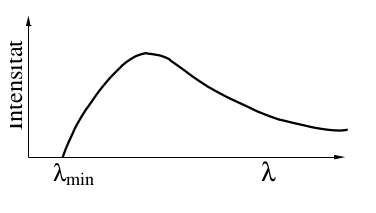
\includegraphics[height=4cm]{kont.png}
  \caption{Kontinuierliches Bremsspektrum.}
  \label{fig:kont}
  \cite{skript}
\end{figure}

Trifft ein beschleunigtes Elektron genau auf ein Hüllenelektron der Anode,
wird dieses Hüllenelektron ausgelöst. Nun kann ein Elektron einer höheren Schale den
freien Platz besetzten, bei dem Übergang wird Röntgenstrahlung der Energie
\begin{equation}
  h \nu=E_n -E_m
\end{equation}
freigesetzt. Da die Energiezustände der Hüllenelektronen quantisiert sind, ist auch die
Energie der Röntgenstrahlung quantisiert. Diese Strahlung ist charakteristisch für das
Anodenmaterial und wird dementsprechend charakteristische Strahlung genannt.
Die einzelnen charakteristischen Linien werden mit $K_{\alpha}, K_{\beta}, L_{\alpha}...$
bezeichnet, wobei $K$,$L$,$M$...die Schale angibt auf dem das Elektron endet, während
der Index angibt von welcher Schale das Elektron kommt. Das charakteristische Spektrum
ist dem Bremsspektrum überlagert.\\

Bei größeren Atomen wird die Coulombanziehung des Kerns durch die anderen Hüllenelektronen
abgeschirmt, deshalb wird eine effektive Kernladungszahl $z_{eff}=z-\sigma$
eingeführt. Damit folgt für die Bindungsenergie eines Hüllenelektrons:
\begin{equation}
  E_n= -R_{\infty}{z_{eff}}^{2}\cdot \frac{1}{n²},
  \label{eqn:Ebindung}
\end{equation}
wobei $\sigma$ die Abschirmkonstante ist, die sich für jedes Elektron unterscheidet.
$R_{\infty}=\SI{13.6}{\eV}$ ist die Rydbergenergie.
Aus \ref{eqn:Ebindung} lässt sich für die Energie $E_{K_{\alpha}}$ der $K_{\alpha}$-Linie
die Formel
\begin{equation}
  E_{K_{\alpha}}=R_{\infty}(z-\sigma_{1})^{2}\cdot\frac{1}{1²}-R_{\infty}(z-\sigma_{2})^{2}\cdot\frac{1}{2²}
  \label{eqn:k}
\end{equation}
herleiten.
Jede charakteristische Linien lässt sich in eine Feinstruktur unterteilen, da
äußere Elektronen aufgrund des Bahndrehimpulses und des Elektronenspins unterschiedlich
viel Energie besitzen. Diese Feinstruktur wird in diesem Versuch jedoch nicht genauer
untersucht.

\subsection{Absorption von Röntgenstrahlung}
Für den Fall, dass die Energie der Röntgenstrahlung unter $\SI{1}{\mega\electronvolt}$ liegt,
sind der Photoeffekt und der Comptoneffekt die dominierenden Effekte.
Mit zunehmender Energie nimmt der Absorptionskoeffizient so lange ab, bis
er plötzlich sprunghaft ansteigt. Dies geschieht genau dann, wenn die Energie der
Röntgenstrahlung gerade größer ist als die Bindungsenergie eines Hüllenelektrons
der inneren Schale ist.

\begin{figure}
  \centering
  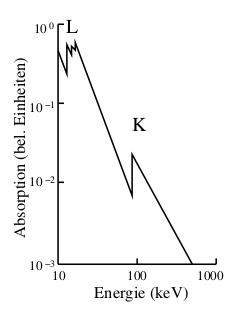
\includegraphics[height=5cm]{kont2.png}
  \caption{Beispielhaftes Spektrum der Absorption.}
  \label{fig:kont2}
  \cite{skript}
\end{figure}
Dieser sprunghafte Anstieg wird als Absoptionskante bezeichnet, diese hat die Lage von
\begin{equation}
  h\nu_{\text{abs}}=E_n - E_{\infty}.
\end{equation}
Die Absoptionskanten werden je nach Schale aus der das Elektron stammt mit
K-, L-, M-,... Absorptionskanten bezeichnet. Diese lassen sich noch weiter in
eine Feinstruktur unterteilen, da die Feinstruktur in diesem Versuch nicht untersucht wird,
wird nicht näher darauf eingegangen.

Um die Abschirmkonstante aus den L-Kanten zu bestimmen wird zunächst die Energiedifferenz
\begin{equation}
  \Delta \text{E}_L = \text{E}_{LII} - \text{E}_{LIII}
\end{equation}
berechnet. Die $\text{E}_{LI}$ Kante wird nicht verwendet, da die Auflösung der
Apparatur nicht hoch genug ist.
Die Berechnung der Abschirmkonstante erfolgt dann durch die Formel
\begin{equation}
  \sigma_L = \text{Z} - \left(\frac{4}{\alpha}\sqrt{\frac{\Delta\text{E}_L}{\text{R}_{\infty}}}-
  \frac{5 \Delta E_L}{R_{\infty}} \right)^{(1/2)}
  \left(1+\frac{19}{32}\alpha^2\frac{\Delta\text{E}_L}{\text{R}_\infty}\right)^{(1/2)} \: ,
  \label{eqn:L}
\end{equation}
wobei $\alpha=7,297353 \cdot 10^{-3}$ die Feinstrukturkonstante bezeichnet.
%In diesem Versuch wird eine Kupferanode verwendet, somit
%können die $Cu_{K_{\alpha}}$ und $Cu_{K_{\beta}}$ -Linien beobachtet werden. Diese sind der
%kontinuierlichen Bremsstrahlung überlagert. Dies ist beispielsweise in Abbildung
%\ref{fig:spektrum} dargestellt.

\subsection{Bragg-Bedingung}

Um die Energie und damit auch die Wellenlänge der Röntgenstrahlung zu bestimmen wird die
Bragg-Bedingung ausgenutzt. Hierbei fällt die Röntgenstrahlung auf einen Kristall und wird an den
Atomen des Kristalls gebeugt, dadurch kommt es zu Interferez. Der Ort an dem konstruktive
Interferenz beobachtet wird, wird Glanzwinkel $\theta$ genannt.
Mathematisch ausgedrückt hat die Bragg-Bedingung folgende Gestallt:
\begin{equation}
  2d\sin(\theta)=n\lambda.
  \label{eqn:bragg}
\end{equation}

\begin{figure}
  \centering
  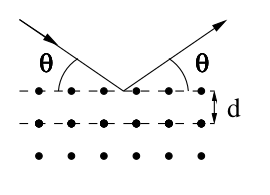
\includegraphics[height=4cm]{bragg.png}
  \caption{Röntgenstrahlung wird an den Atomen des Kristallgitters gebeugt.}
  \label{fig:bragg}
  \cite{skript}
\end{figure}



\section{Vorbereitung}

Zur Vorbereitung auf diesen Versuch wurden Energiewerte sowie zu erwartende Glanzwinkel verschiedener
Metalle ermittelt, um den Messbereich genauer wählen zu können.
Für die Überprüfung der Absorption wurden folgende Daten für Kupfer ermittelt:
\begin{align*}
  Cu-K_{\alpha}-Linie:& \;\;\;E_K=\SI{8,10}{\keV}\;\;\;\;&\theta &=22,7°\\
  Cu-K_{\beta}-Linie:& \;\;\;E_K=\SI{8,92}{\keV}\;\;\;\;&\theta &=20,15°
\end{align*}
\cite{leifi}, \cite{kbeta}.
In Tabelle \ref{tab:tabvor} sind Daten zu finden, die für die Absorptionsmessung
vorbereitet wurden. Es sind hier nur die Metalle aufgelistet, die auch im Versuch
untersucht werden.
\begin{table}[H]
  \centering
   \begin{tabular}{c c c c c}
    \toprule
     & Z & $E_{K}$/\;keV & $\theta_{K}$ /\;° & $\sigma_{K}$ \\
    \midrule
    Zn & 30 & 9,65 & 18,6 & 3,37\\
    Sr & 38 & 16,1 & 11,0 & 3,60\\
    Br & 35 & 13,5 & 13,2 & 3,50\\
    Zr & 40 & 18,0 & 9,8 & 3,62 \\
    \bottomrule
  \end{tabular}
  \caption{Zur Vorbereitung ermittelte Werte der einzelnen Metalle.}
  \label{tab:tabvor}
\end{table}

%Z & $E_{K}$/\; keV & $\theta_{K}$/\; ° & $\sigma_{K}$

